\documentclass[12pt]{article}

\usepackage{amsmath, mathtools}
\usepackage{amsfonts}
\usepackage{amssymb}
\usepackage{graphicx}
\usepackage{colortbl}
\usepackage{xr}
\usepackage{hyperref}
\usepackage{longtable}
\usepackage{xfrac}
\usepackage{tabularx}
\usepackage{float}
\usepackage{siunitx}
\usepackage{booktabs}
\usepackage{caption}
\usepackage{pdflscape}
\usepackage{afterpage}

\usepackage[round]{natbib}

%\usepackage{refcheck}

\hypersetup{
    bookmarks=true,         % show bookmarks bar?
      colorlinks=true,       % false: boxed links; true: colored links
    linkcolor=black,          % color of internal links (change box color with 
    %linkbordercolor)
    citecolor=blue,        % color of links to bibliography
    filecolor=magenta,      % color of file links
    urlcolor=cyan           % color of external links
}

%% Comments

\usepackage{color}

\newif\ifcomments\commentstrue

\ifcomments
\newcommand{\authornote}[3]{\textcolor{#1}{[#3 ---#2]}}
\newcommand{\todo}[1]{\textcolor{red}{[TODO: #1]}}
\else
\newcommand{\authornote}[3]{}
\newcommand{\todo}[1]{}
\fi

\newcommand{\wss}[1]{\authornote{blue}{SS}{#1}}
\newcommand{\hz}[1]{\authornote{magenta}{Author}{#1}}


% For easy change of table widths
\newcommand{\colZwidth}{1.0\textwidth}
\newcommand{\colAwidth}{0.13\textwidth}
\newcommand{\colBwidth}{0.82\textwidth}
\newcommand{\colCwidth}{0.1\textwidth}
\newcommand{\colDwidth}{0.05\textwidth}
\newcommand{\colEwidth}{0.8\textwidth}
\newcommand{\colFwidth}{0.17\textwidth}
\newcommand{\colGwidth}{0.5\textwidth}
\newcommand{\colHwidth}{0.28\textwidth}

% Used so that cross-references have a meaningful prefix
\newcounter{defnum} %Definition Number
\newcommand{\dthedefnum}{GD\thedefnum}
\newcommand{\dref}[1]{GD\ref{#1}}
\newcounter{datadefnum} %Datadefinition Number
\newcommand{\ddthedatadefnum}{DD\thedatadefnum}
\newcommand{\ddref}[1]{DD\ref{#1}}
\newcounter{theorynum} %Theory Number
\newcommand{\tthetheorynum}{T\thetheorynum}
\newcommand{\tref}[1]{T\ref{#1}}
\newcounter{tablenum} %Table Number
\newcommand{\tbthetablenum}{T\thetablenum}
\newcommand{\tbref}[1]{TB\ref{#1}}
\newcounter{assumpnum} %Assumption Number
\newcommand{\atheassumpnum}{P\theassumpnum}
\newcommand{\aref}[1]{A\ref{#1}}
\newcounter{calcnum} %Calculation number
\newcommand{\cthecalcnum}{C\thecalcnum}
\newcommand{\calcref}[1]{C\ref{#1}}
\newcounter{goalnum} %Goal Number
\newcommand{\gthegoalnum}{P\thegoalnum}
\newcommand{\gsref}[1]{GS\ref{#1}}
\newcounter{instnum} %Instance Number
\newcommand{\itheinstnum}{IM\theinstnum}
\newcommand{\iref}[1]{IM\ref{#1}}
\newcounter{reqnum} %Requirement Number
\newcommand{\rthereqnum}{P\thereqnum}
\newcommand{\rref}[1]{R\ref{#1}}
\newcounter{nfreqnum} %Nonfunctional Requirement Number
\newcommand{\rthenfreqnum}{P\thenfreqnum}
\newcommand{\nfrref}[1]{NFR\ref{#1}}
\newcounter{lcnum} %Likely change number
\newcommand{\lthelcnum}{LC\thelcnum}
\newcommand{\lcref}[1]{LC\ref{#1}}
\newcommand\inn{ %math element of symbol
	\mathrel{\ooalign{$\subset$\cr\hfil\scalebox{0.8}[1]{$=$}\hfil\cr}}%
}
\newcommand{\famname}{LoSMS} % PUT YOUR PROGRAM NAME 
%HERE

\usepackage{fullpage}

\begin{document}

\title{Commonality Analysis of a Library of Simplex Method Solvers (\famname{}) 
\wss{Put the name of your library in the title}\hz{done}} 
\author{Hanane Zlitni}
\date{October 4, 2018}

\maketitle

~\newpage

\pagenumbering{roman}

\section{Revision History}

\begin{tabularx}{\textwidth}{p{3cm}p{2cm}X}
	\toprule {\bf Date} & {\bf Version} & {\bf Notes}\\
	\midrule
	December 17, 2018 & 2.0 & Final Draft (includes making the document 
	consistent with the rest of the deliverables)\\
	December 16, 2018 & 1.2 & Applied Dr.~Smith’s Comments\\
	October 13, 2018 & 1.1 & Applied the comments obtained from Jennifer 
	Garner's review\\
	October 4, 2018 & 1.0 & First Draft\\
	\bottomrule
\end{tabularx}

~\newpage
	
\section{Reference Material}

This section records information for easy reference.

\subsection{Table of Units}

This section is not applicable for \famname{}.

\subsection{Table of Symbols}

The table that follows summarizes the symbols used in this document.

\renewcommand{\arraystretch}{1.2}
%\noindent \begin{tabularx}{1.0\textwidth}{l l X}
\noindent \begin{longtable*}{l l p{12cm}} \toprule
\textbf{symbol} & \textbf{unit} & \textbf{description}\\
\midrule 
	$Z$ & - & Optimal solution of the objective function\\
	$Z'$ & - & The negation of the objective function\\
	$R$ & - & The set of real numbers\\
	$N$ & - & The set of natural numbers\\
\bottomrule
\end{longtable*}

\subsection{Abbreviations and Acronyms}

\renewcommand{\arraystretch}{1.2}
\begin{tabular}{l l} 
  \toprule		
  \textbf{symbol} & \textbf{description}\\
  \midrule 
  A & Assumption\\
  C & Calculation \\
  DD & Data Definition\\
  GD & General Definition\\
  GS & Goal Statement\\
  IM & Instance Model\\
  LC & Likely Change\\
  PS & Physical System Description\\
  R & Requirement\\
  SRS & Software Requirements Specification\\
  CA & Commonality Analysis\\
  \famname{} & Library of Simplex Method Solvers\\
  T & Theoretical Model\\
  $s.\;t.$ & Subject to\\
  2D & 2 Dimentional \\
  \bottomrule
\end{tabular}\\

\newpage

\tableofcontents

\listoftables

\listoffigures

~\newpage

\pagenumbering{arabic}

\section{Introduction}

Linear programming is a method to achieve the best possible outcome in a 
mathematical model which is represented by linear relationships. It can also be 
called ``Linear Optimization''.

The simplex method is a linear programming algorithm that is considered one of 
the most popular algorithms which has significant influence in the fields of 
science and engineering (\cite{simplex-popularity}).

\wss{In your introduction it would be nice to say what linear programming
  actually is.}\hz{done.}

The algorithm can be used in a variety of fields and its goal is to make the 
most of the available resources to achieve the optimal solution. For example, 
the simplex method is used in the sand casting process to optimize the sand 
casting parameters to produce the best results (\cite{sand-casting}). Moreover, 
the simplex method was used in chemistry to maximize the yield of a chemical 
reaction (\cite{chemistry}).

Since the simplex method has various applications in different fields, a 
software that facilitates solving objective functions using the simplex method 
for different purposes can be useful.

This commonality analysis (CA) provides detailed documentation of a 
general-purpose program family, called \famname{} (Library of Simplex Method 
Solvers), that solves linear programming problems using the simplex method. The 
reason for choosing this specific algorithm is because of its high efficiency, 
its numerous applications and its influence in various fields including science 
and engineering. The CA template is based on \citet{Smith2006}.

\subsection{Purpose of Document}

The purpose of this document is to formally describe the requirements for the 
development of the \famname{} tool which simplifies obtaining the optimal 
solution of linear programs. Having a thorough and comprehensive documentation 
of this tool would be useful for future use of \famname{}, possible 
enhancements and maintenance.

\subsection{Scope of the Family} 

The scope of \famname{} is limited to solving linear equations using the 
simplex method. The tool supports both maximization and minimization linear 
programs.

\subsection{Characteristics of Intended Reader} 

The intended reader of this document must have basic knowledge of linear 
programming which is typically given to year 3 undergraduate students. The 
intended reader must also have basic knowledge of linear algebra and calculus. 
No technical background is required.

\subsection{Organization of Document}

The document begins by providing a general description of the system, which 
includes potential system contexts, user characteristics and system 
constraints, in Section \ref{SecSystemDescription}. Then, Section 
\ref{Sec_Commonalities} describes the commonalities in the \famname{} program 
family by giving a background overview of the tool, terminology definitions, 
data definitions that are used to build instance models, goal statements and 
theoretical models. Next, Section \ref{Sec_Variabilities} details the 
variabilities in the tool and consists of instance models and assumptions. This 
is followed by the functional and nonfunctional requirements of the \famname{} 
tool in Section \ref{Sec_Requirements} and likely changes in variabilities in 
Section \ref{Sec_LikelyChanges}. Finally, Section \ref{Sec_TraceabilityMatrix} 
visualises the way different sections of this document can be traced to one 
another. \\

\section{General System Description} \label{SecSystemDescription}

This section identifies the interfaces between the system and its environment,
describes the potential user characteristics and lists the potential system
constraints.

\subsection{Potential System Contexts}

\begin{figure}[h!]
	\begin{center}
		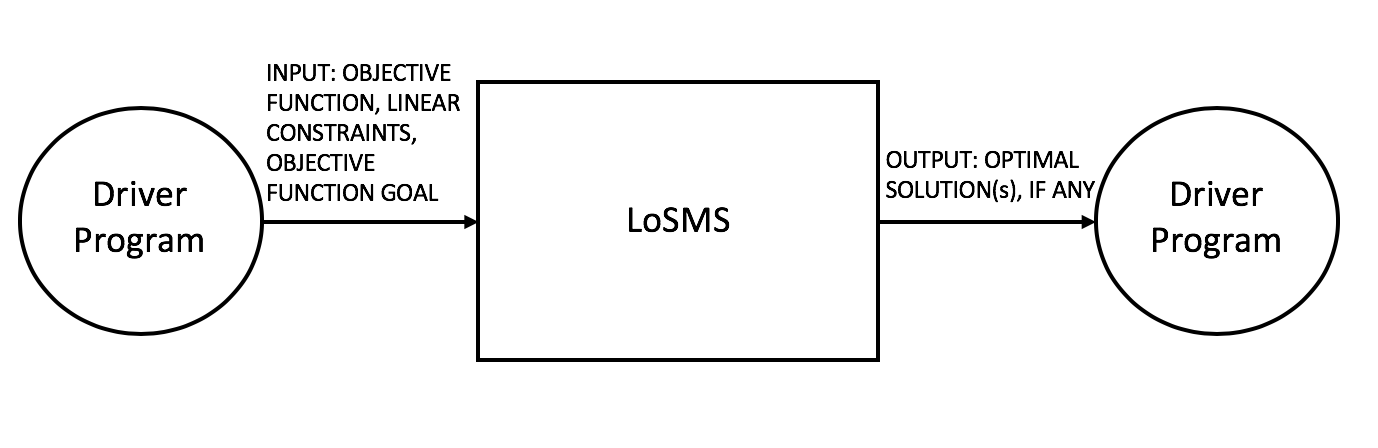
\includegraphics[width=0.9\textwidth, 
		height=0.20\textheight]{system-context}
		\caption{System Context}
		\label{Figure_SystemContext} 
	\end{center}
\end{figure}

\wss{Nice to see the drive program is interacting with your library, and not a
  user.}\hz{thank you.}

Figure~\ref{Figure_SystemContext} describes the system context of \famname{}. 
The user inputs the correct data and \famname{} displays the output, if any.

\begin{itemize}
	\item Driver Program Responsibilities: \wss{Rather than user 
	responsibilities, you should probably discuss the calling programs 
	responsibilities}\hz{done.}
	\begin{itemize}
		\item Input the objective function, linear constraints and the 
		objective function goal.
		\item Handle the case where an input is completely missing.
		\item Handle the case where an input is entered in a wrong format.
	\end{itemize}
	\item \famname{} Responsibilities:
	\begin{itemize}
		\item Handle the case where an input is empty.
		\item Find and display the optimal value of the objective function 
		along with the points where that value occurs (the values of the 
		decision variables), if any.
	\end{itemize}
\end{itemize}

\wss{You say optimal solution, but it is unclear whether you mean the value of
  the optimal value of the objective function, or the optimal value and the
  corresponding values of the decision variables.}\hz{I elaborated in the 
  explanation.}

\subsection{Potential User Characteristics} \label{SecUserCharacteristics}

The end user of \famname{} should have basic knowledge of linear programming  
which is typically given in an operations research course to year 3 
undergraduate students in Mathematics and in some Engineering programs like 
Software Engineering.  \wss{A little more information would be good here.  
Undergraduate students in what programs? What course subject would typically 
cover linear programming - operations research? systems?}\hz{done.}

\subsection{Potential System Constraints}

\famname{} does not have any system constraints.

\section{Commonalities} \label{Sec_Commonalities}

This section begins by providing a general idea about the \famname{} tool, 
followed by terminology and data definitions, goal statements and theoretical 
models.

\subsection{Background Overview} \label{Sec_Background}

\famname{} is a program family that facilitates obtaining the optimal solution 
of linear programs given the objective function and linear constraints. The 
tool can be beneficial for users coming from various fields, including physics 
and chemistry. \\

The following figure visualizes the simplex method in a 2D graph:

\begin{figure}[H]
	\centering
	
\includegraphics[width=0.5\textwidth]{Simplex-description-en.png}
	\caption{Simplex Method 2D Graph}
	\label{FigSimplex}
\end{figure}

\wss{The background section would be a great place to show the ``classic'' 2D
  picture of the simplex method.}\hz{done}

\subsection{Terminology and  Definitions}

This subsection provides a list of terms that are used in the subsequent
sections and their meaning, with the purpose of reducing ambiguity and making it
easier to correctly understand the requirements:

\begin{itemize}
	\item Linear program: An optimization problem where the goal is to minimize 
	or maximize the objective function.
	
	\item Objective function: The function to be minimized or maximized.
	
	\item Objective function goal: The choice of minimizing or maximizing the 
	objective function.
	
	\item Linear constraints: Linear constraints are some of the main inputs 
	needed to solve a linear programming problem. They can be equalities or 
	inequalities. There are two types of linear constraints: \textit{main 
	constraints} (e.g. $2x_1 + 3x_2 \leq 10$) and \textit{non-negativity 
	constraints} (e.g. $x_1, x_2 \geq 0$).
	
	\item Decision variables: They are variables that represent the parameters 
	that the user wishes to optimize, and they are written as: ${x_1}$, 
	${x_2}$, ..., ${x_k}$, where $k \in N$.
	
	\item Entering variable: An entering variable is the entry in the simplex 
	tableau that becomes the pivot instead of a previous entry.
	
	\item Departing variable: A departing variable is the orevious entry in the 
	simplex tableau that was the pivot and got replaced by the entering 
	variable.
	
	\item Feasible solution: The point that satisfies all constraints and sign 
	restrictions.
	
	\item Feasible region: The set of all feasible points.
	
	\item Optimal solution/The optimum: A feasible solution with the maximum 
	value in maximization objective functions or the minimum value in 
	minimization objective functions.
\end{itemize}

\subsection{Data Definitions} \label{sec_datadef}

This section collects and defines all the data needed to build the instance
models. The dimension of each quantity is also given.  
	
~\newline

\noindent
\begin{minipage}{\textwidth}
	\renewcommand*{\arraystretch}{1.5}
	\begin{tabular}{| p{\colAwidth} | p{\colBwidth}|}
		\hline
		\rowcolor[gray]{0.9}
		Number& DD\refstepcounter{datadefnum}\thedatadefnum 
		\label{minToMax}\\
		\hline
		Label& \bf The Negation of a Minimization Linear Program\\
		\hline
		Symbol & $Z'$\\
		\hline
		Equation& $Z' = -Z$\\
		\hline
		Description & 
		To convert the linear program goal from minimization to maximization, 
		negate the minimization function by multiplying it by -1.
		\\
		\hline
		Sources& -\\
		\hline
		Ref.\ By & \iref{minLP}\\
		\hline
	\end{tabular}
\end{minipage}\\

\wss{It is nice to see that IM2 actually does reference DD1.  Good!}\hz{thank 
you (:}

~\newline

\noindent
\begin{minipage}{\textwidth}
	\renewcommand*{\arraystretch}{1.5}
	\begin{tabular}{| p{\colAwidth} | p{\colBwidth}|}
		\hline
		\rowcolor[gray]{0.9}
		Number& DD\refstepcounter{datadefnum}\thedatadefnum 
		\label{simplexTableau}\\
		\hline
		Label& \bf The Simplex Tableau\\
		\hline
		Symbol & sTableau \\
		\hline
		Equation& sTableau = $\begin{bmatrix}
		a_{11} & a_{12} & a_{13} & a_{14} & \dots & b_{1}\\
		a_{21} & a_{22} & a_{23} & a_{24} & \dots & b_{2}\\
		\vdots & \vdots & \vdots & \vdots & \dots & \vdots\\
		\vdots & \vdots & \vdots & \vdots & \dots & \vdots\\
		a_{n1} & a_{n2} & a_{n3} & a_{n4} & \dots & b_{n}	
		\end{bmatrix}$ , where: $a, b \in R$ and $n$ = the row number\\
		\hline
		Description & 
		The simplex tableau is the augmented matrix form that \famname{} 
		creates from the linear program's equations.\\
		\hline
		Sources& \cite{lp-book}\\
		\hline
		Ref.\ By & \iref{maxLP}\\
		\hline
	\end{tabular}
\end{minipage}\\
\wss{I feel like there should be a symbol for the tableau and a 
source.}\hz{done}
~\newline

\noindent
\begin{minipage}{\textwidth}
	\renewcommand*{\arraystretch}{1.5}
	\begin{tabular}{| p{\colAwidth} | p{\colBwidth}|}
		\hline
		\rowcolor[gray]{0.9}
		Number& DD\refstepcounter{datadefnum}\thedatadefnum 
		\label{slackVar}\\
		\hline
		Label& \bf The Slack Variable\\
		\hline
		Symbol & $S_n$\\
		\hline
		Equation& $a_1x_1 + a_2x_2\;{\leq}\;b_n$ becomes $a_1x_1 + a_2x_2 + S_n 
		= b_n$ \\
		\hline
		Description & 
		The slack variable is a variable that represents zero or a positive 
		real number. It is added to the simplex tableau to convert it to the 
		canonical form (see \tref{T_SLPCF}). This can also be called an 
		``artificial variable''.
		\\
		\hline
		Sources& \cite{lp-defs}\\
		\hline
		Ref.\ By & \iref{maxLP}\\
		\hline
	\end{tabular}
\end{minipage}\\

\subsection{Goal Statements}

\noindent Given the objective function, linear constraints and the objective 
function goal, the goal statement of \famname{} is: 

\begin{itemize}
	\item[GS\refstepcounter{goalnum}\thegoalnum \label{goalStatement}:] Use the 
	simplex method to find and output the optimal value of the objective 
	function and the values of the decision variables satisfying all linear 
	constraints and sign restrictions.
\end{itemize}

\wss{Rather than display the optimal solution, say ``output'' the optimal
  solution.  This is a more abstract way to say it.}\hz{done} \wss{As mentioned
  previously, you should be clear on what you mean by the optimal 
  solution.}\hz{done}

\subsection{Theoretical Models} \label{sec_theoretical}

This section focuses on the general equations and laws that \famname{} is based
on.

~\newline

\noindent
\begin{minipage}{\textwidth}
	\renewcommand*{\arraystretch}{1.5}
	\begin{tabular}{| p{\colAwidth} | p{\colBwidth}|}
		\hline
		\rowcolor[gray]{0.9}
		Number& T\refstepcounter{theorynum}\thetheorynum \label{T_SLPCF}\\
	  	\hline
	  	Label&\bf The Canonical Form of a Linear Program\\
	  	\hline
	  	Equation& sTableau = $\begin{bmatrix}
	  	a_{11} & a_{12} & a_{13} & a_{14} & \dots & b_{1}\\
	  	a_{21} & a_{22} & a_{23} & a_{24} & \dots & b_{2}\\
	  	\vdots & \vdots & \vdots & \vdots & \dots & \vdots\\
	  	\vdots & \vdots & \vdots & \vdots & \dots & \vdots\\
	  	a_{n1} & a_{n2} & a_{n3} & a_{n4} & \dots & b_{n}\\
	  	c_{n1} & c_{n2} & c_{n3} & c_{n4} & \dots & 0\\
	  	\end{bmatrix}$\newline
	  	
	  	, where: $a, b, c \in R$ ; $n$ = the row number ; the last row = the 
	  	coefficients of the objective function ; the rest of the rows = the 
	  	coeffiecients of the linear constraints \wss{$a$ and $b$ should have 
	  	the subscripts.  Without the subscripts, they would not have the type 
	  	real, but multidimensional sequences of real.}\hz{I don't really 
        understand which subscripts should be added.}\\
	  	\hline
	  	Description & A linear program is in its canonical form when it 
	  	satisfies the following conditions: \newline
	      \begin{itemize}
	      	\item The objective function is a maximization function
	        
	        \item All constraints are equalities
	        
	        \item All decision variables are greater than or equal to zero.
	      \end{itemize}
      	To convert a simplex tableau to the canonical form, slack variables 
      	(see \ddref{slackVar}) must be added to the tableau.\\
	  	\hline
	  	Source & \cite{lp-defs}\\
	  	\hline
	  	Ref.\ By & \iref{maxLP}, \rref{R_CanonicalForm}\\
	  	\hline
	\end{tabular}
\end{minipage}\\

\wss{The names of functions, like max, should not be in italic font.  You can
  use the following \LaTeX code to change fonts inside an equation: $\text{max }
  Z = ...$}\hz{done.} \wss{Isn't $Z$ usually in lower case in this 
  formula?}\hz{I saw that both upper and lower cases are used online and in 
  text books. I used the upper case because that's what I'm used to when I 
  studied operations research.}

\wss{Do you want to consider using matrix notation for these equations?  I guess
  it depends on how many times you need the equation.  If you are using it
  frequently, the more succinct matrix notation would help.}\hz{You're right, 
  the matrix notation is much better. I will change all occurences of the 
  equations to the matrix form.}

\wss{Isn't this where you want to mention slack variables?}\hz{done.}

\hz{Note: Instead of having two theoretical models for the standard and 
canonical forms, I merged them into one under the name of canonical form 
because I noticed that they aren't differentiated online and in text books. So 
I thought that there's no need to do that here.}

~\newline

\noindent
\begin{minipage}{\textwidth}
	\renewcommand*{\arraystretch}{1.5}
	\begin{tabular}{| p{\colAwidth} | p{\colBwidth}|}
		\hline
		\rowcolor[gray]{0.9}
		Number& T\refstepcounter{theorynum}\thetheorynum \label{T_pivoting}\\
		\hline
		Label&\bf Pivoting in an Augmented Matrix\\
		\hline
		Equation&$\begin{bmatrix}
		a_{11} & a_{12} & a_{13} & \dots & b_{1}\\
		\vdots & \vdots & \vdots & &\vdots\\
		a_{n1} & a_{n2} & a_{n3} & \dots & b_{n}	
		\end{bmatrix}$ , where: $a \in R$ \newline \newline
		Let $R_i$ and $R_j$ be any two rows in the matrix, $i, j \in N$: 
		\newline
		Pivoting includes one or more of the following operations:
		\begin{itemize}
			\item Row switching: $R_i \xleftrightarrow{} R_j$
			
			\item Row addition: $R_i$ + $R_j$
			
			\item Multiplying a row by a non-zero constant: $kR_i$ ; 
			$k \neq 0$
		\end{itemize} \\
		\hline
		Description & 
		Pivoting is the process of performing what's similar to Gaussian 
		elimination with row operations to clear the entries of the pivot 
		column (set them to 0).\newline
		
		The element that performs the pivoting operation is called the 
		``pivot''. It is determined by finding the minimum ratio between the 
		entries in the pivot column and the ones in the same row in the 
		constants column (the last column). This is done to ``guarantee that 
		the new basis obtained after the pivot step will also be a feasible 
		basis''.\\
		\hline
		Source & \cite{lp-book}\\
		\hline
		Ref.\ By & \iref{maxLP}\\
		\hline
	\end{tabular}
\end{minipage}\\

\wss{The information on T3 doesn't actually tell me what pivoting is.  You have
  just defined elementary row operations, not why you would do them.}\hz{That's 
  true. I added an explanation for the actually pivoting process. Thank you.}

\section{Variabilities} \label{Sec_Variabilities} 

This section describes the variabilities in the \famname{} tool and details the 
instance models, assumptions and variabilities in the calculation and the 
output.

\subsection{Instance Models} \label{sec_instance}   

This section transforms the documented problem into one which is expressed in 
mathematical terms.

~\newline

\noindent
\begin{minipage}{\textwidth}
	\renewcommand*{\arraystretch}{1.5}
	\begin{tabular}{| p{\colAwidth} | p{\colBwidth}|}
		\hline
		\rowcolor[gray]{0.9}
		Number& IM\refstepcounter{instnum}\theinstnum \label{maxLP}\\
		\hline
		Label& \bf The Simplex Method for Solving Linear Programs: Maximization 
		Functions\\
		\hline
		Input& 
		\begin{enumerate}
			\item Max objective function in the following form: 
			\newline$max\;Z=\;c_{1}x_1 + c_{2}x_2 + ... + c_{k}x_k$
			
			\item Linear constraint(s) in the following form: 
			\newline$a_{11}x_1 + a_{12}x_2 + ... + a_{nm}x_k\;{\leq}\;b_n$
			\newline$x_1, ..., x_k\;{\geq}\;0$
		\end{enumerate} , where: $c, a, b \in R$ ; $k, n, m \in N$\\
		\hline
		Output& The optimal solution $Z$ and the points $x_i$ where $Z$ occurs 
		(the values of the decision variables) \wss{I'm surprised you 
		just want $Z$.  Don't you also want the $x_i$ values that give you 
		$Z$?}\hz{Yes. I added it.}\\
		\hline
		Description& The purpose of this instance model is to provide details 
		about solving linear programs that intend to maximize a parameter. The 
		steps to solve a maximization problem are:
		\begin{enumerate}
			\item Convert linear program to its canonical form using slack 
			variables.
			
			\item Set up the simplex method tableau.
			
			\item Perform pivoting.
			
			\item Set up the new simplex tableau.
			
			\item Repeat steps 2-4 until there are no negative numbers in the 
			bottom row of the tableau.
			
			\item The optimal solution $Z$ is found in the basic feasible 
			solution derived from the final tableau.
		\end{enumerate}
		\\
		\hline
		Sources& \cite{lp-defs}\\
		\hline
		Ref.\ By & \iref{minLP}, Section \ref{sec_Calculation}, 
		\rref{R_Calculate}\\
		\hline
	\end{tabular}
\end{minipage}\\

~\newline

\noindent
\begin{minipage}{\textwidth}
	\renewcommand*{\arraystretch}{1.5}
	\begin{tabular}{| p{\colAwidth} | p{\colBwidth}|}
		\hline
		\rowcolor[gray]{0.9}
		Number& IM\refstepcounter{instnum}\theinstnum \label{minLP}\\
		\hline
		Label& \bf The Simplex Method for Solving Linear Programs: Minimization 
		Functions\\
		\hline
		Input& 
		\begin{enumerate}
			\item Min objective function in the following form: 
			\newline$min\;Z=\;c_{1}x_1 + c_{2}x_2 + ... + c_{k}x_k$
			
			\item Linear constraint(s) in the following form: 
			\newline$a_{11}x_1 + a_{12}x_2 + ... + a_{nm}x_k\;{\leq}\;b_n$
			\newline$x_1, ..., x_k\;{\geq}\;0$
		\end{enumerate} , where: $c, a, b \in R$ ; $k, n, m \in N$\\
		\hline
		Output& The optimal solution $Z$ and the points $x_i$ where $Z$ occurs 
		(the values of the decision variables)\\
		\hline
		Description& The purpose of this instance model is to provide details 
		about solving linear programs that intend to minimize a parameter. The 
		steps to solve a minimization problem are:
		\begin{enumerate}
			\item Convert the minimization linear program to a maximization 
			linear program by finding $Z'$ defined in \ddref{minToMax}.
			
			\item Solve \iref{maxLP}.
		\end{enumerate}
		\\
		\hline
		Sources& \cite{lp-defs}\\
		\hline
		Ref.\ By & Section \ref{sec_Calculation}, \rref{R_Calculate} \\
		\hline
	\end{tabular}
\end{minipage}\\

\wss{You have missed the notion of binding time.  You could have family members
  where the number of equations are fixed at design time.  This information
  could be hard-coded into a family member.  I don't think you need to add this
  now, but you could clarify that the size variabilities are all left to
  run-time.}\hz{clarified in 6.3.}

\wss{You could have mentioned the ``covering'' variation (see the Wikipedia page
  for Linear Programming.}

\subsubsection*{Derivation of the Simplex Method}{
	The origin of the simplex method is detailed in \cite{simplex-origin}. 
}

\subsection{Assumptions} \label{Assumptions}

\begin{itemize}
	\item[A\refstepcounter{assumpnum}\theassumpnum \label{A_objFunSpace}:] The 
	objective function $Z \in R$.
	
	\item[A\refstepcounter{assumpnum}\theassumpnum \label{A_inequalities}:] If 
	the linear constraints are inequalities, they are of type less than or 
	equal to. This is to ensure that there are no negative variables.
	
	\item[A\refstepcounter{assumpnum}\theassumpnum \label{A_NonNegative}:] It 
	is assumed that all linear programs have the non-negativity constraint 
	(i.e. the decision variables are greater than 0), even if the 
	non-negativity constraint is not present in a linear program.
	
	\item[A\refstepcounter{assumpnum}\theassumpnum \label{A_GoalMax}:] The 
	default linear program goal is maximization.
\end{itemize}

\subsection{Calculation} \label{sec_Calculation}

\famname{} has some variabilities in its calculations. For instance, 
\iref{maxLP} is solved when the linear program is a maximization problem, while 
\iref{minLP} is solved when the linear program is a minimization 
problem. \\

Moreover, the size of the linear program (i.e. the number of linear 
constraints and decision variables) varies and it is left to be determined at 
run-time.

\wss{It would be better if you phrased these as variabilities.  You could also
  have mentioned the variabilities I mentioned above.}\hz{done.}

\subsection{Output} \label{sec_Output}

Similar to its calculations, \famname{} has variabilities in its output, as 
well. The library currently outputs the optimal solution $Z$ and the values of 
the decision variables $x_i$. However, with a small change, the library can 
just output $Z$ or $x_i$, depending on what's desired. Furthermore, the format 
of the output varies. The library can output the solution to the screen and 
write it to a file. It can also be expanded in the future to accomodate more 
output format options.

\wss{You have more output variabilities than this.  You have the decision on
  whether the output includes the $x$ values, or not.  You could output to the
  screen, or to a file, or to memory.  The format of the output could be a
  variability.}\hz{I made changes to this section. Thank you for the 
  clarification.}

\section{Requirements} \label{Sec_Requirements}

This section provides the functional requirements, the business tasks that the
software is expected to complete, and the nonfunctional requirements, the
qualities that the software is expected to exhibit.

\subsection{Functional Requirements}

\noindent 
\begin{itemize}
	\item[R\refstepcounter{reqnum}\thereqnum \label{R_Inputs}:] The \famname{} 
	tool shall read the objective function, linear constraints and the 
	objective function goal from the user.
	
	\item[R\refstepcounter{reqnum}\thereqnum \label{R_HandleInputErrors}:] The 
	\famname{} tool shall verify that all inputs are valid and satisfy 
	\aref{A_objFunSpace} and \aref{A_inequalities}.
	
	\item[R\refstepcounter{reqnum}\thereqnum \label{R_DisplayErrorMsg}:] If 
	there are invalid inputs, the \famname{} tool shall display a corresponding 
	message to the user.
	
	\item[R\refstepcounter{reqnum}\thereqnum \label{R_CanonicalForm}:] The 
	\famname{} tool shall convert the linear program to its canonical form 
	(\tref{T_SLPCF}).

	\item[R\refstepcounter{reqnum}\thereqnum \label{R_Calculate}:] The 
	\famname{} tool shall find the optimal solution of the linear program and 
	the points where it occurs by solving \iref{maxLP} or \iref{minLP}, 
	depending on the objective function goal.
	
	\item[R\refstepcounter{reqnum}\thereqnum \label{R_Output}:] The \famname{} 
	tool shall display the optimal solution and the points where it occurs to 
	the user, if any.
	
	\item[R\refstepcounter{reqnum}\thereqnum \label{R_OutputError}:] If the 
	given linear program does not have an optimal solution, the \famname{} 
	tool shall display a corresponding message to the user.
\end{itemize}

\subsection{Nonfunctional Requirements}

\subsubsection*{Usability}

\noindent 
\begin{itemize}
	\item[NFR\refstepcounter{nfreqnum}\thenfreqnum \label{NFR_usability}:] It 
	shall 
	take at most 10 minutes for the user to learn to use the \famname{} tool.
\end{itemize}

\subsubsection*{Portability}

\begin{itemize}
	\item[NFR\refstepcounter{nfreqnum}\thenfreqnum \label{NFR_portability}:] 
	The 
	\famname{} tool shall be operable in Windows, Mac and Linux operating 
	systems.
\end{itemize}

\subsubsection*{Accuracy}

\begin{itemize}
	\item[NFR\refstepcounter{nfreqnum}\thenfreqnum \label{NFR_accuracy}:] The 
	relative error of the output of the \famname{} tool shall be less than 
	0.2. 
\end{itemize}

\subsubsection*{Correctness}

\begin{itemize}
	\item[NFR\refstepcounter{nfreqnum}\thenfreqnum \label{NFR_correctness}:] 
	The difference between the output of \famname{} and MatLab for the same 
	linear program shall be less than 10\%.
\end{itemize}

\subsubsection*{Performance}

\begin{itemize}
	\item[NFR\refstepcounter{nfreqnum}\thenfreqnum \label{NFR_performance}:] It 
	shall take no more than 3 seconds for \famname{} to calculate the solution.
\end{itemize}

\subsubsection*{Stability}

\begin{itemize}
	\item[NFR\refstepcounter{nfreqnum}\thenfreqnum \label{NFR_stability}:] The 
	\famname{} tool shall handle a heavy load of inputs and not crash.
\end{itemize}

\section{Likely Changes} \label{Sec_LikelyChanges} 

\noindent 
\begin{itemize}
	\item[LC\refstepcounter{lcnum}\thelcnum\label{LC_inequalities}:] The 
	support for greater than or equal to inequalities in the linear constraints.
	
	\item[LC\refstepcounter{lcnum}\thelcnum\label{LC_moreAlgorithms}:] The 
	support for additional linear programming algorithms like the criss-cross 
	and interior point algorithms. \wss{You could name some other algorithms, 
	like the criss-cross algorithm, or interior point methods.}\hz{done}
\end{itemize}

\section{Traceability Matrices and Graphs} \label{Sec_TraceabilityMatrix}

The purpose of a traceability matrix is to visualise the way different 
components of this CA are dependent on one another. Every time a component in a 
row is changed, the component in the corresponding column marked with an "X" 
may have to be changed as well.  Table~\ref{Table_traceability1} shows the 
traceability between the data definitions, theoretical models, instance models, 
assumptions and the calculation.

\begin{table}[h!]
	\centering
	\begin{tabular}{|c|c|c|c|c|c|c|c|c|c|c|c|}
		\hline        
		& \ddref{minToMax} & \ddref{simplexTableau} & \ddref{slackVar} & 
		\tref{T_SLPCF} & \tref{T_pivoting} & \iref{maxLP} & 
		\iref{minLP} & \aref{A_objFunSpace} & \aref{A_inequalities} \\
		\hline
		\ddref{minToMax} 	    &   &   &   &   &   &   & X &   &  \\
		\hline
		\ddref{simplexTableau}  &   &   &   &   &   & X &   &   &  \\ 
		\hline
		\ddref{slackVar} 		&   &   &   &   &   & X &   &   &  \\ 
		\hline
		\tref{T_SLPCF} 	  		&   &   &   &   &   & X &   &   &  \\ 
		\hline  
		\tref{T_pivoting} 		&   &   &   &   &   & X &   &   &  \\ 
		\hline
		\iref{maxLP} 	  		&   &   &   &   &   &   & X &   &  \\ 
		\hline
		\iref{minLP}   			&   &   &   &   &   &   &   &   &  \\ 
		\hline
		\aref{A_objFunSpace}	&   &   &   &   &   &   &   &   &  \\
		\hline 
		\aref{A_inequalities} 	&   &   &   &   &   & X &   &   &  \\
		\hline
	\end{tabular}
	\caption{Traceability Matrix Showing the Dependencies between Components of 
	this CA}
	\label{Table_traceability1}
\end{table}

\newpage

\bibliographystyle {plainnat}
\bibliography {../../refs/References}

\newpage

\section{Appendix}

	This section provides additional content related to this commonality 
	analysis.

\subsection{Symbolic Parameters}

There are no symbolic parameters used in this document.

\end{document}